%!TEX root = ../main.tex
%%%%%%%%%%%%%%%%%%%%%%%%%%%%%%%%%%
% Links:
%
% Difficulty: Companies: 
%%%%%%%%%%%%%%%%%%%%%%%%%%%%%%%%%%


%\begin{figure} \centering 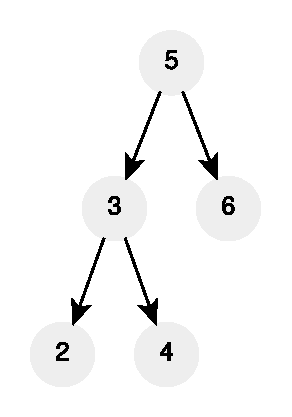
\includegraphics[width=\textwidth]{sources/max_triplet/images/example1}
%   \caption[Sample short cpation]{Sample Caption}. \label{fig:max_triplet:example1} \end{figure}

\chapter{Max triplet sum}
\label{ch:max_triplet}
\section*{Introduction}

\section{Problem statement}
\begin{exercise}
\label{example:max_triplet:exercice1}
Write a function that, given an array $I$ of length $n$, returns the maximum value obtainable by
summing $3$ distinct elements of $I$: $I_i$, $I_j$ and $I_k$ such that $ 0 \leq i < j < k \leq n-1$
and $ I_i < I_j < I_k $.


	%example1
	\begin{example}
		\label{example:max_triplet:example1}
		\hfill \\
		Given $I = \{2, 5, 3, 1, 4, 9\}$ the function returns $16$. The max value of $16$ is
		obtainable by summing together the elements of $I$ at indices: $0$,$1$ and $5$ : $I_0 +
		I_1+I_5=2+5+9= 16$.
		
		Notice that there is another way of obtains the max sum of $16$, that is by using the
		elements at indices $2$,$4$ and $5$: $I_2 + I_4+I_5=3+4+9= 16$.
	\end{example}

	%example2
	\begin{example}
		\label{example:max_triplet:example2}
		\hfill \\
		Given $I = \{3,2,1\}$ the function returns $-1$ as there is no valid triplet in $I$.		
	\end{example}
	
		\begin{example}
			\hfill \\
			Given $I = \{1,3,2\}$ the function returns $-1$ as there is no valid triplet in $I$.
			\label{ex:max_triplet:example2}	
		\end{example}

	\begin{example}
		\hfill \\
		Given $I = \{1,2,3\}$ the function returns $6$. There is only one valid triplet in $I$.
	\label{ex:max_triplet:example3}
	\end{example}
\end{exercise}

\section{Clarification Questions}

\begin{QandA}
	\begin{questionitem} \begin{question} Is it guaranteed that $I$ contains at least three elements?  \end{question} 	 
    \begin{answered}
		\textit{No. When $n < 3$ the function should return $-1$.}
	\end{answered} \end{questionitem}
	\begin{questionitem} \begin{question} Is it guaranteed the answer to fit a standard \inline{int}?  \end{question} 	 
    \begin{answered}
		\textit{Yes you can assume the the answer always fits a standard $4$-bytes \inline{int}}
	\end{answered} \end{questionitem}
\end{QandA}

\section{Discussion}
\label{max_triplet:sec:discussion}
The problem is asking us to find the largest possible sum obtainable by summing up three distinct
elements of $I$ with the additional constraint that when ordered according to their indices they
form a sorted sequence. You can form such a triplet by selecting an element at index $i$, then
another element at index $j$ that it appears after and it is larger than the element at position $i$
and finally, a third element at index $k$ which appears after and it is larger than the element at
index $j$.

\section{Brute-force}
\label{max_triplet:sec:bruteforce}
We can solve this problem trivially in a brute-force manner by trying all possible triplets of
ordered indices $i < j <k$ and keep track of the triplet yielding the maximum value. Three simple
nested loops are enough to implement this idea, as shown in Listing
\ref{list:max_triplet_bruteforce}. The time complexity of this approach is $(O(|I|^3)$ which is far
from being optimal. The space complexity is $O(1)$ as no additional space is used.

\lstinputlisting[language=c++, caption={Cubic time complexity bruteforce solution.},label=list:max_triplet_bruteforce]{sources/max_triplet/max_triplet_solution1.cpp}


\section{Precalculation and Binary Search}
The cubic time complexity approach discussed in Section \ref{max_triplet:sec:bruteforce} can be
dramatically improved if we approach the problem a little differently. Imagine we would be able to
efficiently calculate $L_j$ and $G_j$ for an element at index $j$ where:
\begin{enumerate}
	\item $L_j$ is the \textbf{largest} value among any of the elements of $I$ appearing at any
	index \textbf{smaller} than $j$ and it is \textbf{smaller} than $I_j$;
	\item $G_j$ is the \textbf{largest} value among any of the elements of $I$ appearing at any
	index \textbf{higher} than $j$ and it is \textbf{larger} than $I_J$.
\end{enumerate}
When these values are available we can calculate the value of the largest sum obtainable by any
triplet having $I_j$  as the middle element. The triplet $(L_j, I_j, G_j)$ yield the largest sum
as if that was not the case it would mean that either existed a larger element than $L_j$ that is smaller
than $I_j$ in any of the positions before $j$ or that existed an element that is larger than $G_j$
in any of the positions after $j$. 
Both of these two scenarios are impossible  because $L_j$ is by
definition the largest element that is smaller than $I_j$ and appears before index $j$  and
similarly,  $G_j$ is defined to be the largest element appearing after index $j$ and that is larger
than $I_j$.

We can use this fact to calculate the answer to this problem by looping over $I$ and for each
element $I_j$ calculate $L_j+ I_j+ G_j$. The largest of the sums calculated this way is the final
answer. But how can we calculate $L_j$ and $G_j$ for $I_j$?

$L_j$ can be calculated efficiently by keeping a sorted list of all the values appearing before
index $j$ and use binary search to find $L_j$ in the list while $G_j$ can be precalculated in a
similar fashion to what we have done for the problem in Chapter \ref{ch:greatest_right} where we loop
from the right to the left of $I$ and we keep track of the largest element ($M$) seen so far. If $M$ is larger
then the element we are currently examining ($I_x$) then $M$ is also the largest element larger than $I_x$ appearing after $x$.
If not, it means that $I_x$ is the largest element so far, and that $I_x$ does not have any larger element on its right: thus $M = I_x$ (see Section \ref{sec:greatest_right:linear} and Listing \ref{list:greatest_right_final1}).
\lstinputlisting[language=c++, caption={$O(nlog(n))$ solution to the max triplet sum problem.},label=list:max_triplet]{sources/max_triplet/max_triplet_solution2.cpp}